
Now we have an idea how accurate the cluster expansions is, we can use it to calculate the thermodynamic properties of the \Gls{TFI} model. The sampling of points was explained in \cref{sec:phase_diag}. As a reference, \cref{2dtisingphasediag} is shown once more in \cref{2dtisingphasediag2}
\begin{figure}[!htbp]
    \center
    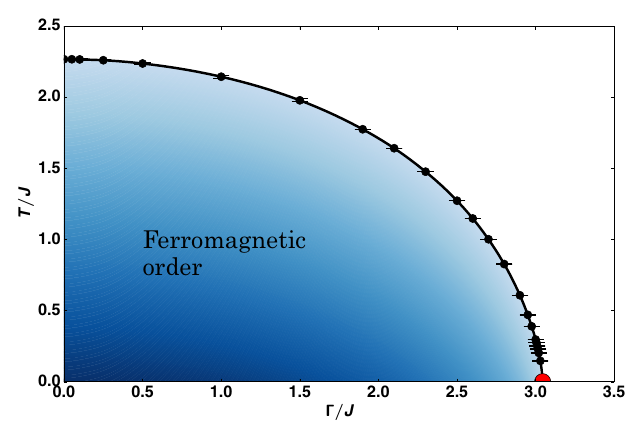
\includegraphics[width=\textwidth]{Figuren/phsyics/2disingphase.png}
    \caption{Phase diagram for 2D \Gls{TFI} model. Figure taken from \cite{Hesselmann2016}.}
    \label{2dtisingphasediag2}
\end{figure}
At the relevant temperature, an order 5 series expansion without loops is sufficient. This keeps the bond dimension small and hence the environment can be computed faster with \Gls{VUMPS}.

\subsection{Classical Ising phase transition}

\begin{figure}[!htbp]
    \center
    \includegraphics[width=\textwidth]{Figuren/phasediag/g0/Full.pdf}
    \caption{ Data collapse for $g=0$ phase transition of \Gls{TFI} Model. }
    \label{fig:phase:g0:full}
\end{figure}
\begin{figure}[!htbp]
    \center
    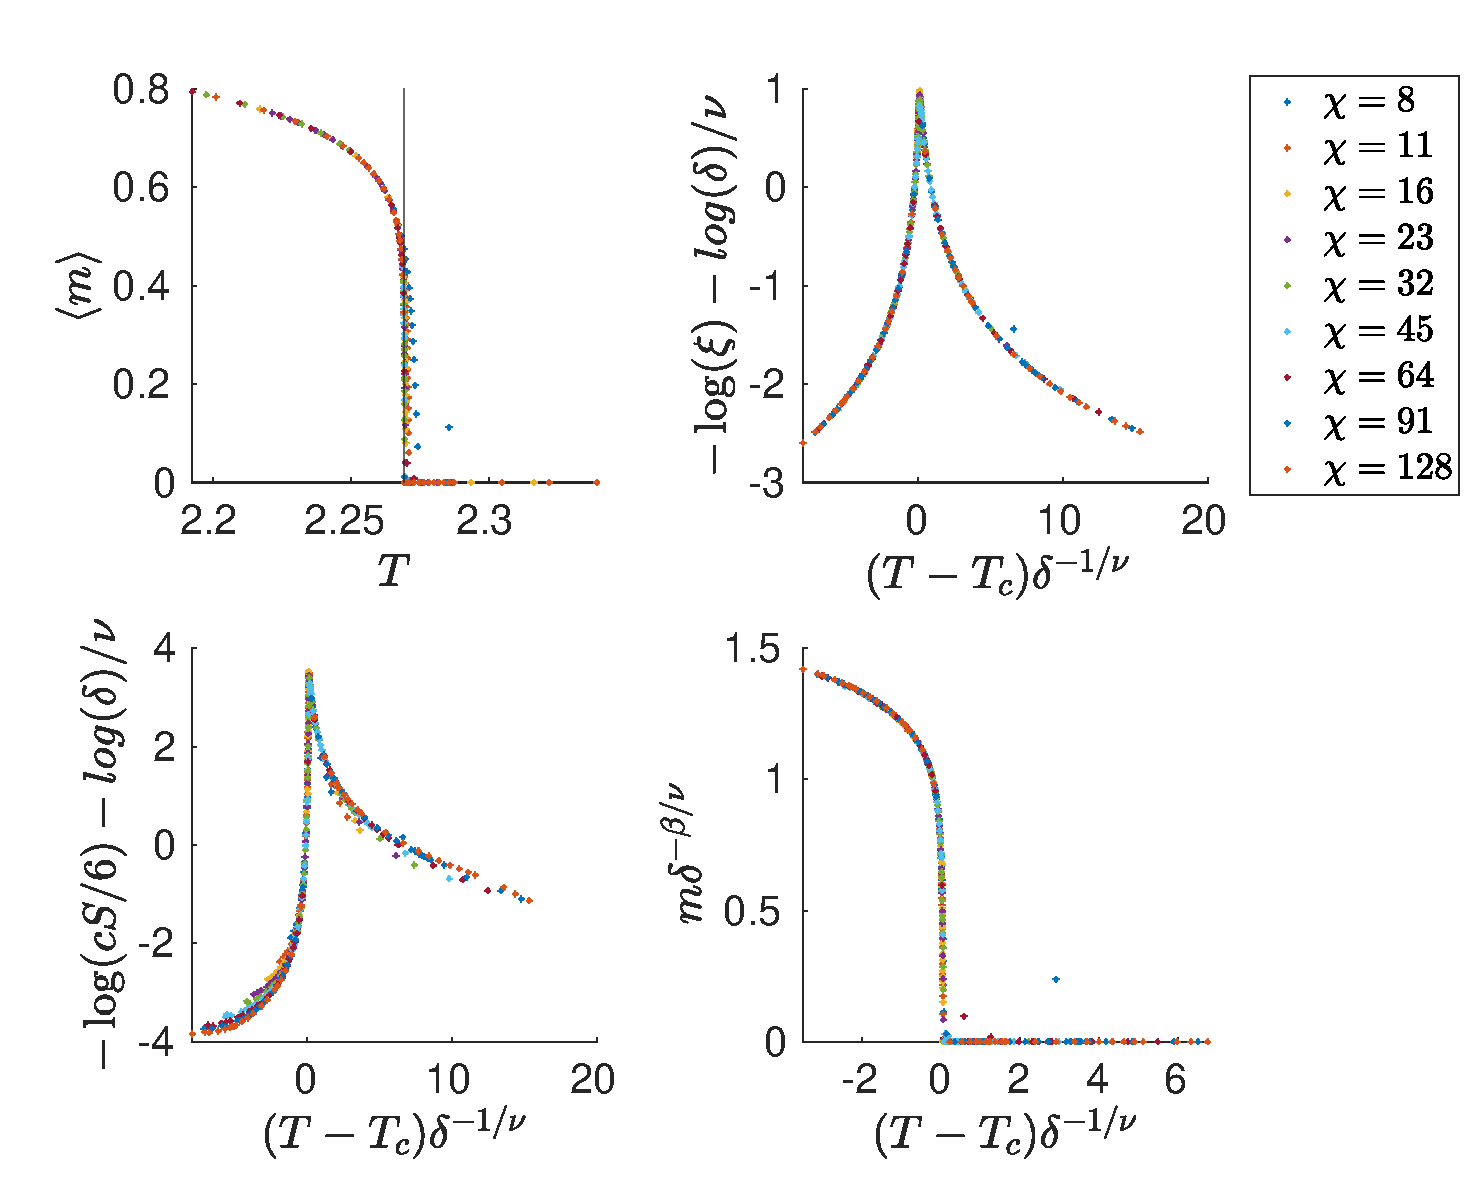
\includegraphics[width=\textwidth]{Figuren/phasediag/g0/zoomed.pdf}
    \caption{ Data collapse for $g=0$ phase transition of \Gls{TFI} Model. Data points are taken from $T \in \left[ T_c -0.08, T_c +0.08 \right]$ }
    \label{fig:phase:g0:zoomed}
\end{figure}

The classical Ising model on a square lattice has an exact solution. Onsager calculated the critical temperature to be $T_c = \frac{2 J}{k \ln(1+\sqrt{2}) } \approx 2.69185 J/k$.  The units are normalised with $J=k=1$ in the remainder of this chapter. A test for the construction is to simulate this phase transition (see \cref{subsec:qphasediag}) and compare the fitted  results. The simulated data points are shown in \cref{fig:phase:g0:full}. Each of the figures has 4 different subplots. The left upper corner shows m vs T. For low T, there is clearly a non-zero macroscopic magnetisation, while high T has a zero expectation value as expected. The other three plots show the data collapse of the finite-size scaling of the entanglement entropy $S$, the correlation length $\xi$ and the magnetisation $m$. $\delta$ is the Marek gap, a measure for the system size as explained in \cref{subsec:fss}. \todo{New figure with entropy formula fixed 6S/c instead of cS/6} Near criticality, they collapse well, but away from the critical point there is quite some systematic variation. The reason is shown in \cref{fig:crit:qtran}. Only in some limited range around the critical region, the universal scaling holds. A more zoomed in version is shown in \cref{fig:phase:g0:zoomed}. Clearly, the data collapses a lot better as expected.

In fact, the data collapses so well that the critical exponents and the temperature could be determined with the given data. The numerical fit (with starting point away from  critical temperature), results in a numerical value of $T_c = 2.691(9) $.

\subsection{g=2.5 phase transition}

\begin{figure}[!htbp]
    \center
    \includegraphics[width=\textwidth]{Figuren/phasediag/g25/Full.pdf}
    \caption{ Data collapse for $g=2.5$ phase transition of \Gls{TFI} Model. }
    \label{fig:phase:g25:full}
\end{figure}

\begin{figure}[!htbp]
    \center
    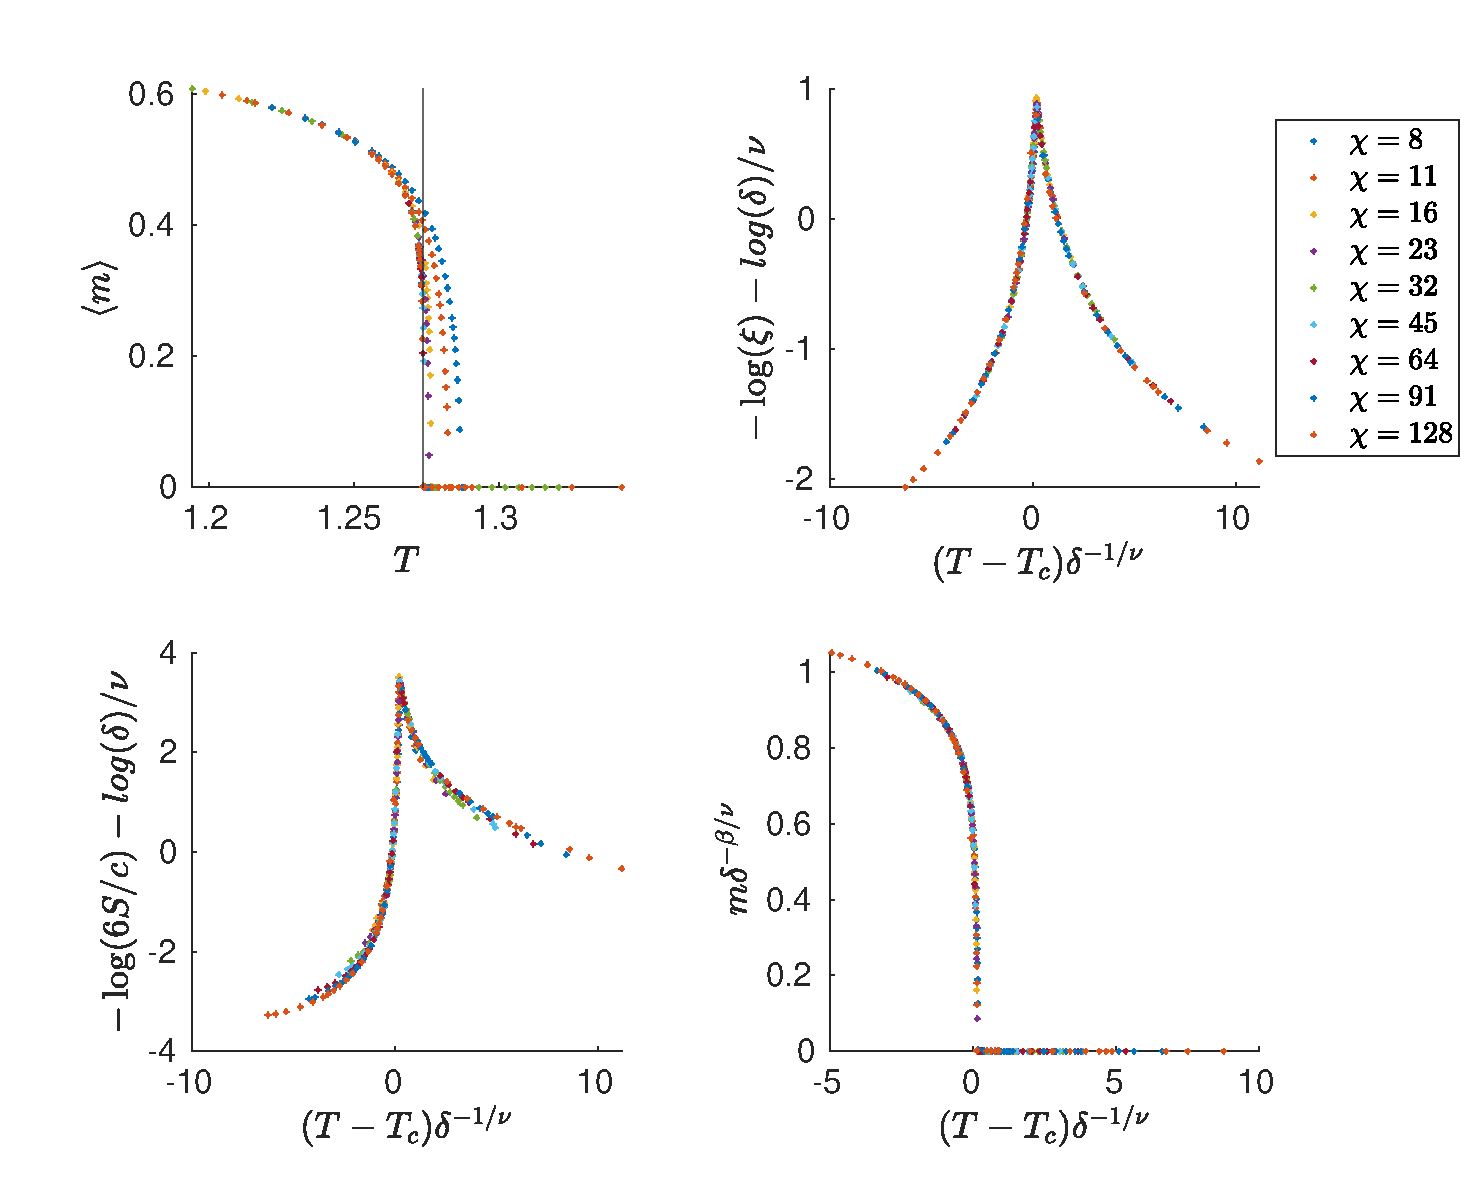
\includegraphics[width=\textwidth]{Figuren/phasediag/g25/zoomed.pdf}
    \caption{ Data collapse for $g=2.5$ phase transition of \Gls{TFI} Model. Data points are taken from $T \in \left[ T_c -0.08, T_c +0.08 \right]$. }
    \label{fig:phase:g25:zoomed}
\end{figure}

The previous example simulated the classical 2D Ising model. The question is whether this result will carry on into the quantum regime. The results for the full phase diagram are shown in \cref{fig:phase:g25:full} and points in the direct neighbourhood of the phase transition are shown in \cref{fig:phase:g25:zoomed}, similar to the classical case. Of course, quantitative details are different: the phase transition happens at $T\approx 1.274$ and the maximum magnetisation is lower than 1, in accordance to \cref{2dtisingphasediag}. The variation of m around the critical temperature for different bond dimensions is much higher. This is not necessarily a problem, as this gives better data for the finite-size scaling.
There is no known analytical expression for the critical temperature. With quantum Monte Carlo techniques, a value of $T_c=1.2737(6)$ is obtained, while state-of-the-art \Gls{TN} techniques provide a value of $T_c=1.2737(2)$ \cite{Czarnik2019}. With the series expansion from this paper and \Gls{VUMPS}, $T_c=1.2736(6)$, indicating that this faithfully captures the physics. To put his into context: the directly calculated error $\epsilon^{2}$  at $T=1.2$ was around $0.006$. This result was achieved for a PEPO with bond dimension 21 (order 5, no loops).

\subsection{T=0.7 quantum phase transition}\label{tphasetranssubsec}

\begin{figure}[!htbp]
    \center
    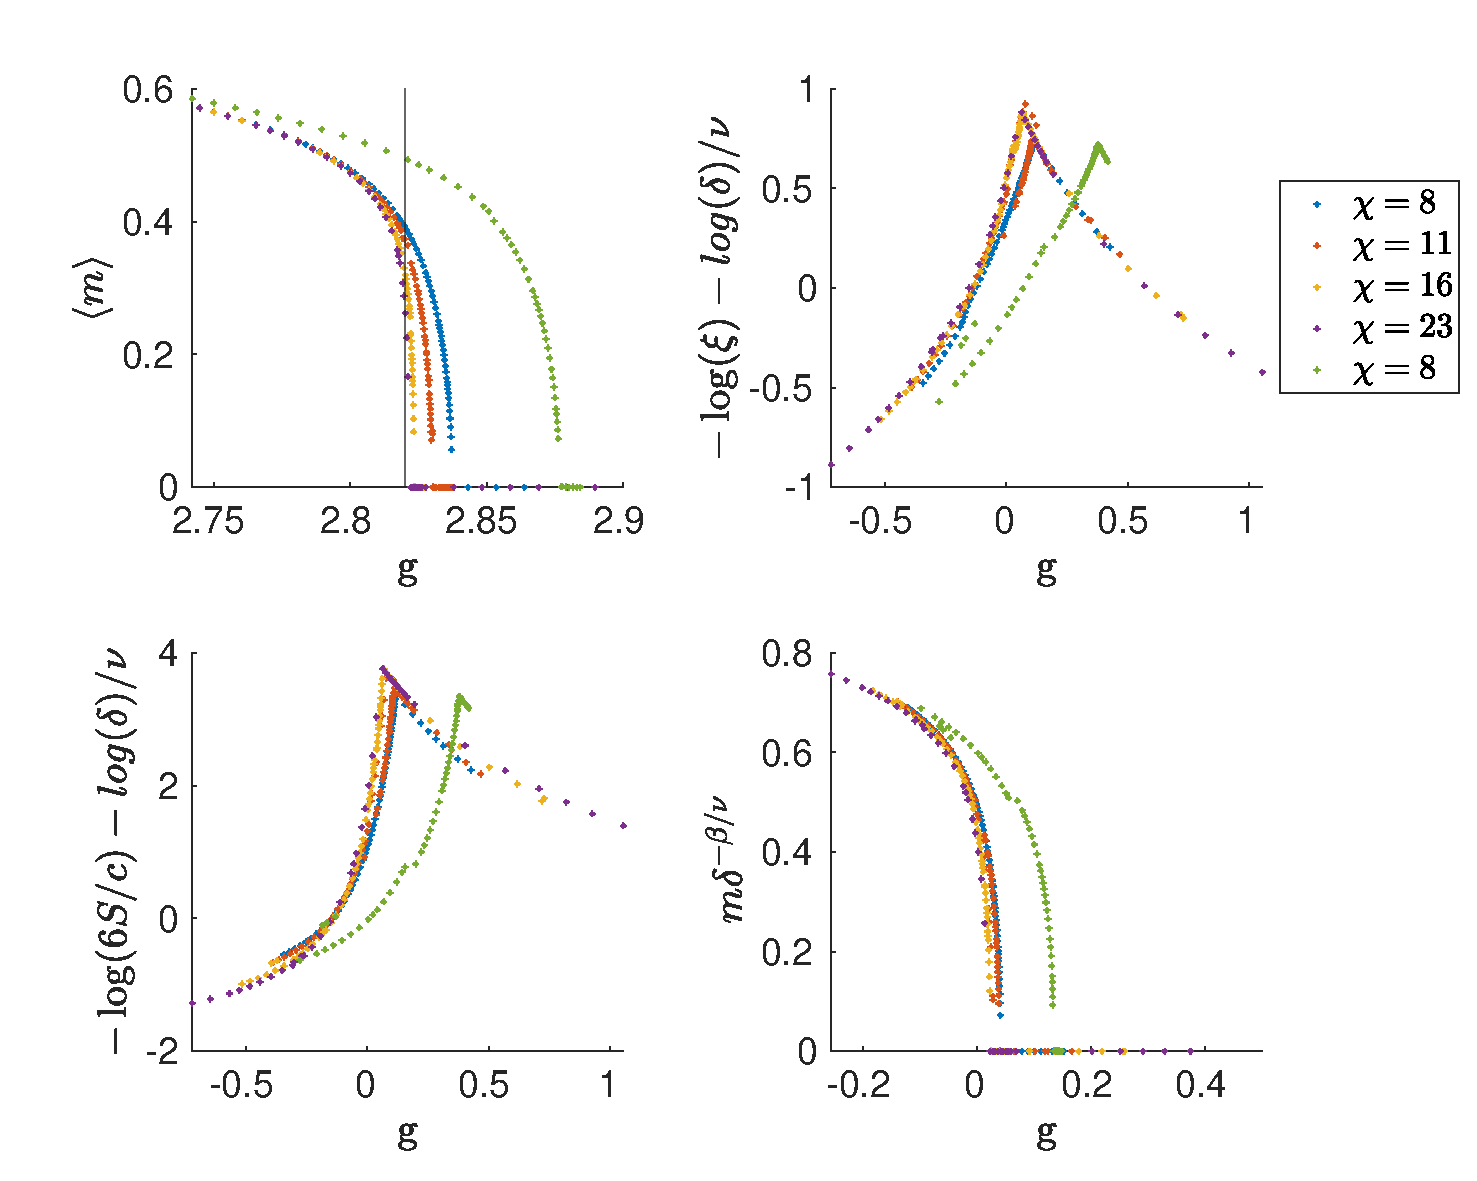
\includegraphics[width=\textwidth]{Figuren/phasediag/t07/full.pdf}
    \caption{Results for $T=0.7$ phase transition. The green points are a truncated order 6 construction, the others order 5.  }
    \label{fig:phase:t07:full}
\end{figure}

\begin{figure}[!htbp]
    \center
    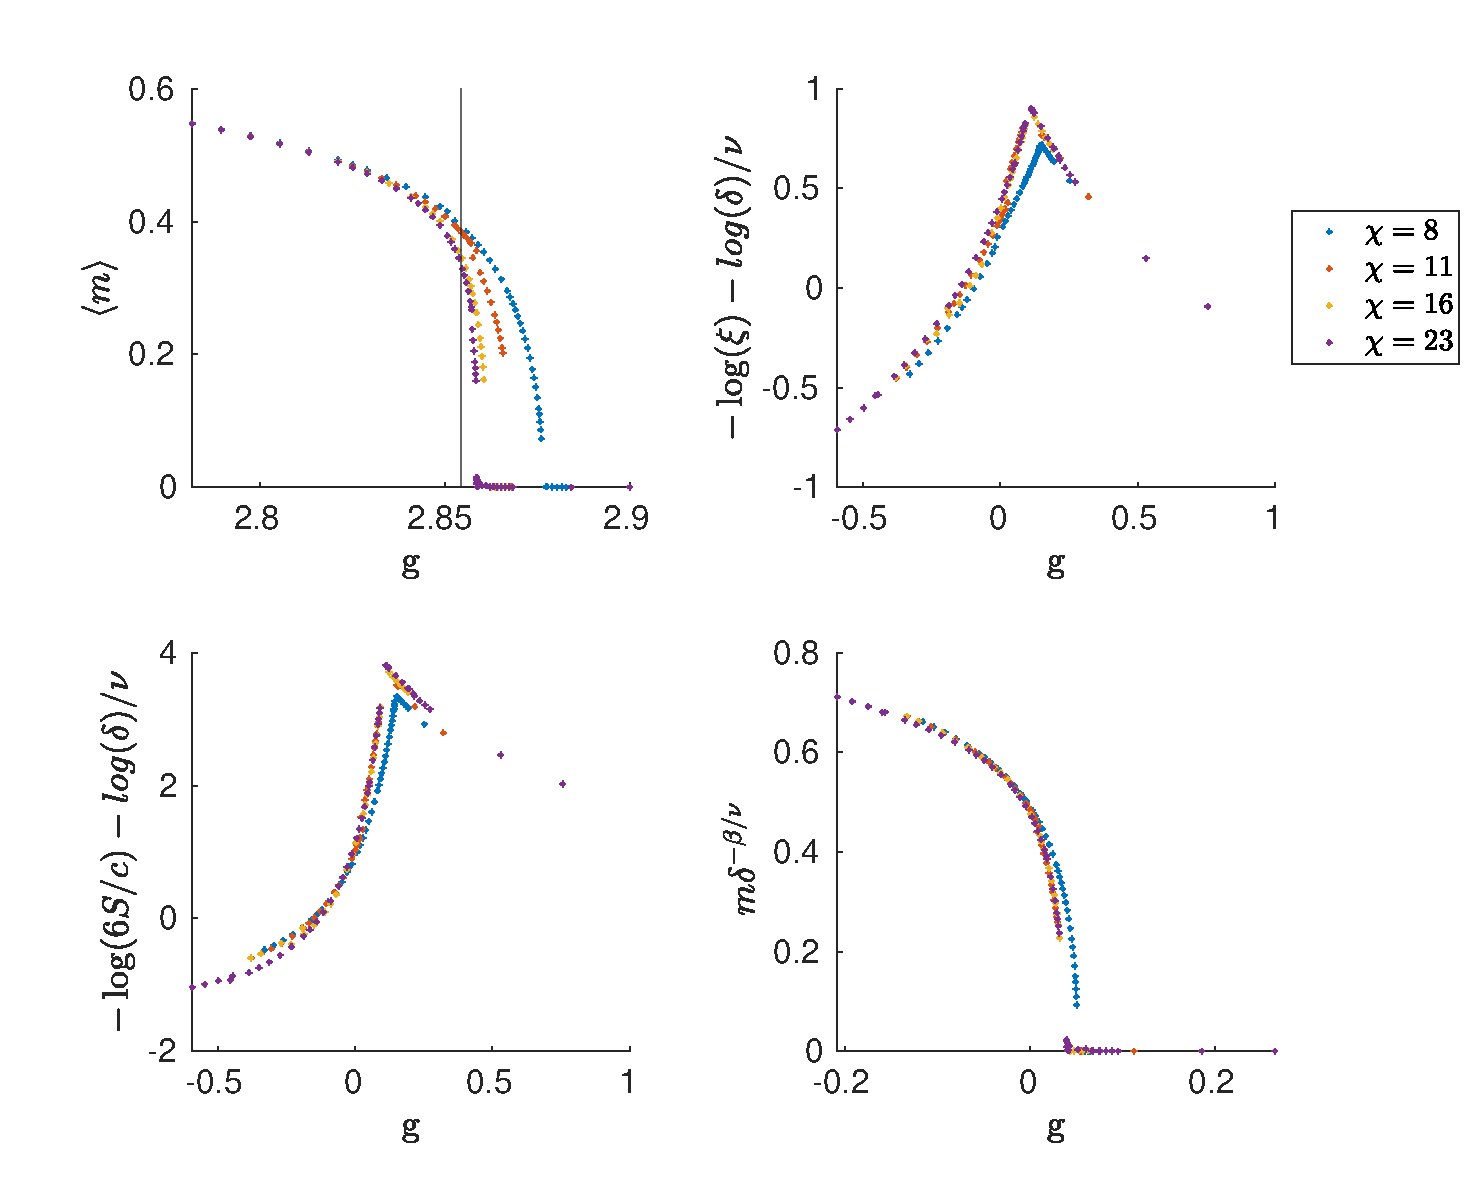
\includegraphics[width=\textwidth]{Figuren/phasediag/t07/zoomed2.pdf}
    \caption{Results for $T=0.7$ phase transition. The cluster expansion is of order 6.}
    \label{fig:phase:t07:full2}
\end{figure}

Up until now, the phase diagram in \cref{2dtisingphasediag2} was explored at constant g in function of T, but of course there is also a transition at constant T and varying g.  T = 0.7 is chosen. The results are shown in \cref{fig:phase:t07:full}. Clearly, the results do not collapse as well as for the other models. The reason is that the order of the expansion is not high enough. The green curve is order 6, where virtual level is truncated to dimension 20. The others are order 5. Both include loop contributions, as opposed to the previous results. The green and blue curve both have \Gls{MPS} bond dimension $\chi=8$, but predict quite different magnetisation for large g. This shows that for $g>0.7$, order 5 is not sufficient any more.
A more accurate version is shown in \cref{fig:phase:t07:full2}. Here, all the cluster expansions are of order 6 with a total bond dimension of ($D = 1+4+16+20$) instead of ($D = 1+4+16$). The results, fitted without $\chi=8$ due to obvious finite-size effects, show a much better collapse.

\subsection{Tricritical point}\label{subsec:tricrit}

Now that we know the critical transversal field can be determined, all the tools are present to extrapolate the tricritical point, indicated by a red dot in \cref{2dtisingphasediag2}. To achieve this, the following scaling relation can be used
\begin{equation}
    T_c = \left| g_c-g_{c,q} \right|^{z \nu_{3D}} .
\end{equation}
Near the critical point, the critical temperature $T_c$ and the critical transversal field $g_c$ are related to each other by the value of the quantum critical point $g_{c,q}$ and critical exponent $z=1$ and $\nu_{3D} \approx 0.62998$ \cite{Hesselmann2016}. This could perfectly be done, given enough computation time to calculate for many temperatures the critical transversal field with a finite-size scaling, similar to \cref{tphasetranssubsec}. Possibly, also a scaling in truncation dimension D for the cluster expansion is needed.

\subsection{Going beyond}
With all the built machinery to construct cluster expansions, it is logical to calculate the phase diagram with increased precision.

\subsubsection{Higher order}

Going to higher order (i.e. longer linear chains) and adding the single loop contribution works well. The bond dimension of the largest virtual level (3 in this case) can be truncated in the construction. The linear and nonlinear solver find the least squares solution to the problems. Care has to be taken in order to not violate one of the conclusions in 1D: never construct a longer chain than the previously fully solved one. For instance if the bond is truncated to 10, the linear chains can be constructed up till order 4. This means \cref{eq:cross_terms:order4} can be added but not \cref{eq:cross_terms:order5}, because the longest chains are order 5. Level 5 can still be constructed and contracted easily, but virtual level 3 has a bond dimension of 64. Compared to the previous bond dimensions (1,4 and 16) this is quite large and needs to be truncated.

\subsubsection{Loops and extensions}\label{subsec:results:loops_and_ext}
Adding loops decreases the direct error. But there is also a surprising result: all possible loop extensions result in a higher error when the environment is calculated in the thermodynamic limit. The fluctuation of the magnetisation increases drastically. With increasing bond dimension $\chi$, this is somewhat better but still not good enough.
The question is whether this is a result of a failing cluster expansion, or the inability of VUMPS to calculate the correct environment. During my thesis, my focus has largely been on the first case. After all, the framework was completely built from scratch and errors happen, and there is no guarantee that the series even converges. But introduction of very strict variants, such as the generalization to type E, where left/upper extension have level a and the right/lower extensions are of type a'
\begin{equation}
    \vcenter{ \hbox{  \pepob{5}{3}{{
                        "-","-","-","-",
                        "-","a","$\alpha$","-",
                        "-","-","$\alpha$","-"}}{{
                        "-","-",
                        "-","-",
                        "-","$\alpha$",
                        "-","$\alpha$",
                        "-","-"}}{{
                        1,1,1,1,1,
                        1,0,0,0,1,
                        1,1,0,0,1}} }} \\
    \vcenter{ \hbox{  \pepob{5}{3}{{
                        "-","-","-","-",
                        "-","0","$\alpha$","-",
                        "-","-","$\alpha$","-"}}{{
                        "-","-",
                        "-","-",
                        "a'","$\alpha$",
                        "-","$\alpha$",
                        "-","-"}}{{
                        1,1,0,1,1,
                        1,1,0,0,1,
                        1,1,0,0,1}} }} ,
\end{equation}
also introduce these fluctuations in the calculated magnetisation.
The \Gls{VUMPS} procedure comes with 2 implicit assumptions. Firstly, in \cref{subsec:vumps_below_alt} the procedure for finding $B$ from below was explained. In the case tested here, the PEPO is rotationally invariant and real. Solving the same equations but with complex tensors, results in wrong magnetisation. For models like Heisenberg, complex tensors are needed to solve the rotationally invariant equations. Switching to complex tensors has no effect on the direct error measures. This suggests the used method for finding B was incorrect. Implementing the suggested solution in \cref{subsec:vumps_below_alt} would come at no extra cost: the tensor is exactly rotation invariant and hence the fixed point form below is automatically known in this case.  A second assumption made during this thesis is that the wave function can be represented by a 1 by 1 unit cell. Despite efforts made, the multisite version \cite{Nietner2020} doesn't seem to produce sensible results, even for PEPO's where the 1 by 1 unit cell does give the right results. It's clear that more research is needed here. One way to locate the problem would be to use another algorithm to contract the network, such as corner transfer matrix renormalization group (CTMRG) as used in  \cite{Czarnik2019}, or even using the single site \Gls{VUMPS} algorithm combined with blocking:

\begin{equation}
    \vcenter{ \hbox{  \pepob{4}{4}{{
                        "","-","",
                        "","","",
                        "","","",
                        "","-","",}}{{
                        "","-","",
                        "","","",
                        "","","",
                        "","-","",}}{{
                        1,4,4,1,
                        4,0,0,4,
                        4,0,0,4,
                        1,4,4,1}} }} \cong  \vcenter{ \hbox{  \pepob{3}{3}{{
                        "","",
                        "","",
                        "","",}}{{
                        "","","",
                        "","","",}}{{
                        1,4,1,
                        4,0,4,
                        1,4,1}} }}
\end{equation}

\subsubsection{Better extrapolation}\label{sssec:better_Extrap}

The spirit behind finite-size scaling is to calculate more with the data available. In \cref{subsec:fss}, 2 additional variations were suggested. One is to account for the subleading finite-size corrections, the other to change the way of calculating $\delta$.

\paragraph{Subleading corrections}
Introducing subleading corrections requires 4 parameters for each fitted universal function: $\omega$, $\phi$, $c$ and $d$ from \cref{ea:subleadparam}. Compared to the one parameter $T_c$ or $g_c$, this is a lot and can be used to make many graphs collapse into a single graph. The analysis in \cite{Wang2006} carefully estimates the error made with the fitting procedure. A similar amount of rigour would be required to fully trust the results. Nevertheless, fitting with subleading corrections results in critical temperatures close to the ones fitted without, and the subleading exponents are close to 1, as expected from the subleading series expansion.

\paragraph{ Choice  $\delta$  }

Different choices of $c_i$ in \cref{eq:cit_delta} are possible to construct $\delta$.  Variational optimisation was done as suggested in \cite{Nietner2020}. Both the x- and y-axis should be normalised, because depending on $\delta$ the scale changes. If the scale is based on the outer points, there is a flaw in the fitting procedure.  The variational minimum goes to a point where at least for one point $\delta$ is extremely close to 0, and hence everything on the x-axis except that point is pinched together, resulting in a very small relative error. Therefore, it is better to normalise according to the points at e.g. the 25th percentile and 75th percentile of the range on the  axis. This improves the collapse, but is not clear how this carries over to the predicted  $T_c$ or $g_c$.

\subsection{Conclusion}

The conclusion from the direct results in \cref{sec:results2d} seems to carry over to a lattice in the thermodynamic limit very well. Comparison with the critical temperatures from literature confirmed that this method is able to approximate the operator $\exp(-\beta \hat{H})$ accurately, even for a cluster expansion of order 5 without loops. This has only a bond dimension of 21, enabling the use of larger \Gls{VUMPS} bond dimensions $\chi$.
The path for determining a value for the tricritical, an important test  to compare this method to the literature, is clear and mostly requires more precise data. With this data, and careful analysis of the end results, the techniques of \cref{sssec:better_Extrap} could be used to improve  the results further. The results also indicate that the current procedure to determine the magnetisation with \Gls{VUMPS}, and in particular the question of how to close the \Gls{VUMPS} environment from below as introduced in \cref{subsec:vumps_below_alt}, deserves some closer attention in the future.